\documentclass{beamer}

\usepackage[utf8]{inputenc}
\usepackage[T1]{fontenc}

\usepackage[english]{babel}
\usepackage{amsmath}
\usepackage{cleveref}
\usepackage{amssymb}
\usepackage{mathtools}

%%Numbers, expectation
\newcommand{\N}{\mathbb{N}}
\newcommand{\E}{\mathbb{E}}
\renewcommand{\P}{\mathbb{P}}
\newcommand{\Var}{\mathbb{V}}
\newcommand{\R}{\mathbb{R}}
\newcommand{\D}{\mathcal{D}}
\newcommand{\B}{\mathcal{B}}
\newcommand{\Dh}{\D_h}
\renewcommand{\phi}{\varphi}
\newcommand*\diff{\mathop{}\!\mathrm{d}} % integral

%% mathoperator
\DeclareMathOperator*{\argmax}{arg\,max}
\DeclareMathOperator*{\argmin}{arg\,min}
\DeclareMathOperator*{\dom}{dom}
\DeclareMathOperator*{\sign}{sign}
\DeclareMathOperator*{\diag}{diag}

\DeclareMathOperator*{\Cov}{Cov}
\DeclareMathOperator*{\Cor}{Corr}
\DeclareMathOperator*{\Id}{Id}

%proximal operator
\newcommand{\prox}[3][]{\operatorname{prox}^{#1}_{#2}\left(#3 \right)}

\usepackage{xcolor}

%% sort citations by increasing number
\usepackage[sort,nocompress]{cite}

\usepackage{graphicx}% http://ctan.org/pkg/graphicx
\graphicspath{{../figures/}{../../figures}{../../memes}} %Setting the graphicspath
\usepackage{caption,subcaption}

\usepackage{tikz}
\usepackage{pgfplots}
\usetikzlibrary{backgrounds}
\usetikzlibrary{intersections}
\usepgfplotslibrary{fillbetween}

% \usepackage[right]{showlabels}


%%
\theoremstyle{plain}
\newtheorem{prop}{Proposition}[section]
\newtheorem{algo}{Algorithm}[section]
\newtheorem{assumption}{Assumption}
\theoremstyle{remark}
\newtheorem{remark}{Remark}[section]

% cref
\crefname{assumption}{Assumption}{Assumptions}
\crefname{equation}{}{}

\usepackage{autonum}

\usepackage{bm} %% bold math symbols

\usepackage{bbm} %% for \mathbbm{1}


% algorithmic environment
\usepackage{algorithm}
\usepackage[noend]{algpseudocode}

% for some reason this was required on one void linux installation (but not the other)
\usepackage{sansmathaccent}
\pdfmapfile{+sansmathaccent.map}

\author{Axel Böhm}

% shows which section we're in
\usetheme{Darmstadt}

% page number
\setbeamertemplate{footline}[frame number]
\setbeamercolor{page number in head/foot}{fg=gray}


% display things like onslide or visible already before but grayed out
\setbeamercovered{transparent}

% set the itemize item symbol as a diamond
\setbeamertemplate{itemize item}{$\diamond$}
% set the itemize subitem symbol as a triangle
\setbeamertemplate{itemize subitem}{$\blacktriangleright$}

% set the enumerate item symbol as a roman numbers
\setbeamertemplate{enumerate item}{(\roman{enumi})}


\author{Axel Böhm}

% shows which section we're in
\usetheme{Darmstadt}

% page number
\setbeamertemplate{footline}[frame number]
\setbeamercolor{page number in head/foot}{fg=gray}


% display things like onslide or visible already before but grayed out
\setbeamercovered{transparent}

% set the itemize item symbol as a diamond
\setbeamertemplate{itemize item}{$\diamond$}
% set the itemize subitem symbol as a triangle
\setbeamertemplate{itemize subitem}{$\blacktriangleright$}

% set the enumerate item symbol as a roman numbers
\setbeamertemplate{enumerate item}{(\roman{enumi})}

\usepackage{changepage}
% https://openai.com/blog/deep-double-descent/

\title{Gradient Descent under strong convexity}
\date{\today}

\begin{document}
\maketitle
\frame{\tableofcontents}

\section{Introduction}%

\begin{frame}
  \frametitle{How fast can we go?}

  \begin{itemize}
    \item So far we explored different smoothness properties.
    \item Error decreased with $1/k$ or $1/\sqrt{k}$
    \item call these rates sublinear
    \item Linear rate means
          \begin{equation}
            Err(x_{k}) \le \frac{C}{\exp(k)}
          \end{equation}
          or
          \begin{equation}
            Err(x_{k+1}) \le q Err(x_k)
          \end{equation}
          with $q<1$.
  \end{itemize}
\end{frame}


\begin{frame}
  \frametitle{Linear convergence}
  \begin{figure}[ht]
    \centering
    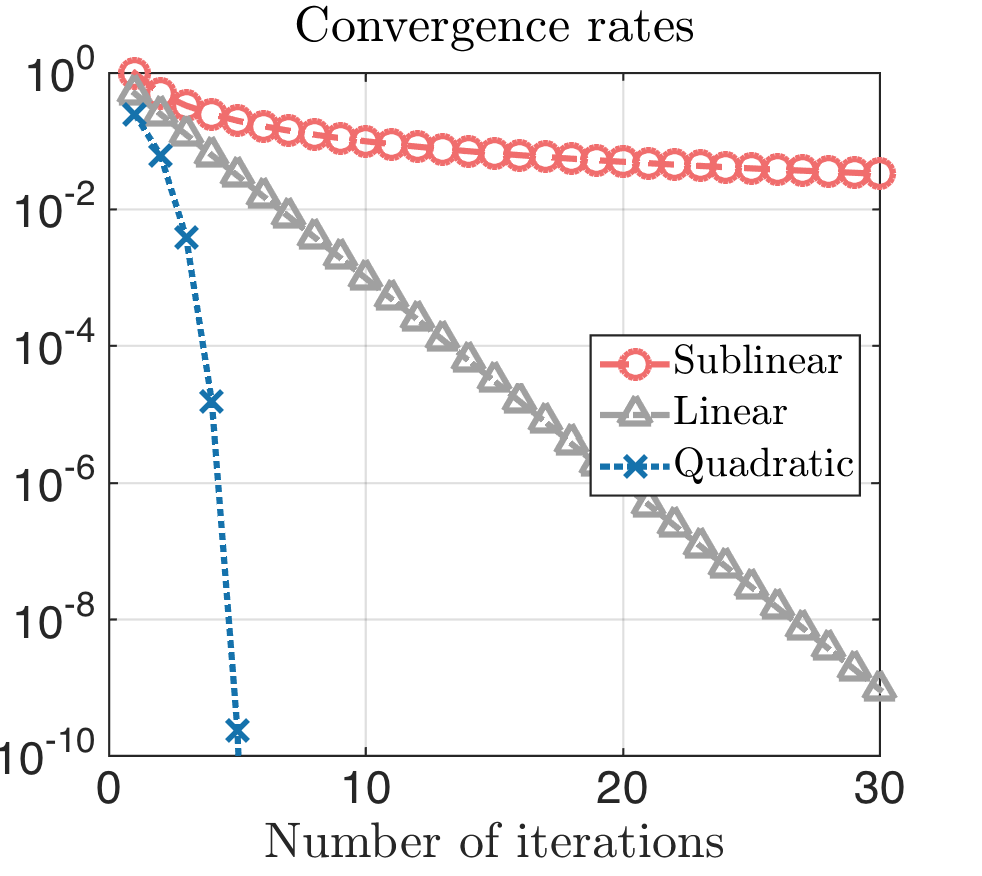
\includegraphics[width=\textwidth,height=0.8\textheight,keepaspectratio]{convergence_rates}
    % \caption{\label{fig:label} }
  \end{figure}
\end{frame}


\begin{frame}
  \frametitle{Example}

  \begin{itemize}
    \item Consider $f(x) = x^2$. Clearly, $f$ is $L=2$ smooth.
          \begin{itemize}
            \item So we can pick $\alpha=1/L = 1/2$ for GD:
                  \begin{equation}
                    x_{k+1} = x_k - \frac12 \nabla f(x_k) = x_k -x_k = 0.
                  \end{equation}
            \item Converges \textbf{in one step!}
          \end{itemize}
    \item Same $f(x)=x^2$, but is also $L=4$ smooth.
          \begin{itemize}
            \item So we can pick $\alpha=1/L = 1/4$ for GD:
                  \begin{equation}
                    x_{k+1} = x_k - \frac14 \nabla f(x_k) = x_k -\frac12 x_k = \frac12 x_k.
                  \end{equation}
            \item Converges \textcolor{blue}{exponentially}
                  \begin{equation}
                    f(x_k) = f\left(\frac{x_0}{2^k}\right) = \frac{1}{2^{2k}} x_0^2.
                  \end{equation}
           \end{itemize}
  \end{itemize}

\end{frame}


\begin{frame}
  \frametitle{Strongly convexity}

  \begin{center}
    \textcolor{blue}{``Not too flat.''}
  \end{center}


  \begin{block}[Recall]
    Let $f: \R^d \to \R$ be a differentiable function, then we say $f$ is $\mu$-strongly convex if
    \begin{equation}
      f(y) \ge f(x) + \langle \nabla f(x), y-x \rangle + \frac{\mu}{2} \Vert y-x \Vert^2, \quad \forall x,y.
    \end{equation}
  \end{block}

\end{frame}

\begin{frame}
  \frametitle{Strong convexity}
  \begin{center}
    \textcolor{blue}{Can be lowe bounded by a quadratic.}
  \end{center}
  \begin{figure}[ht]
    \centering
    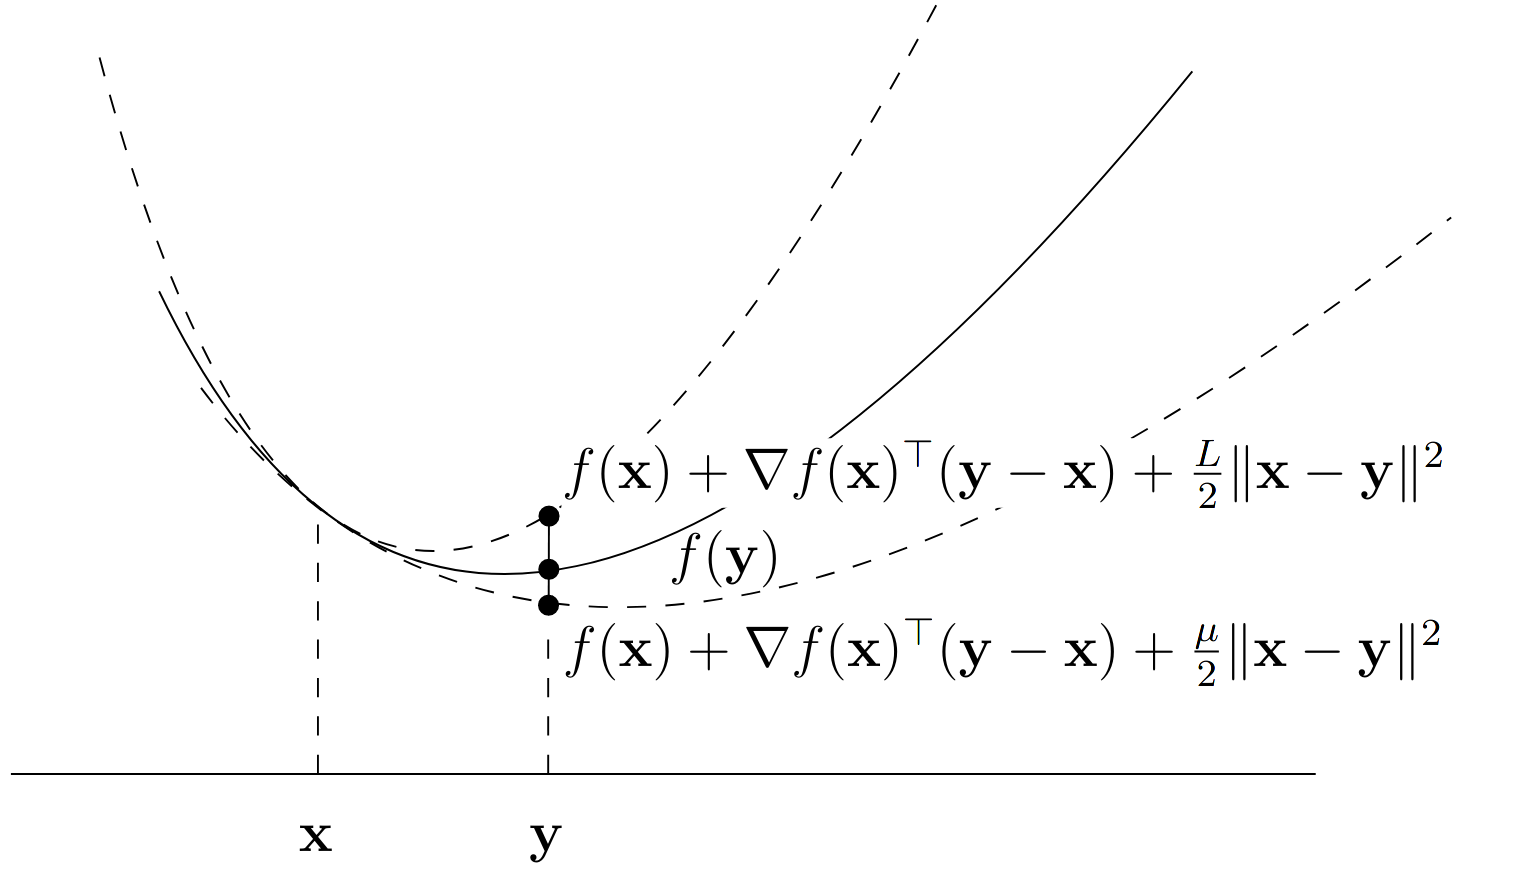
\includegraphics[width=\textwidth,height=\textheight,keepaspectratio]{strongly_convex}
    % \caption{\label{fig:label} }
  \end{figure}

\end{frame}

\section{Convergence analysis}%
\label{sec:}

\begin{frame}
  \frametitle{Smooth strongly convex functions}

  \begin{theorem}
    Let $f:\R^d \to \R$ be $L$-smooth and $\mu$-strongly convex. Then GD with stepsize $\alpha=1/L$ and arbitrary starting point $x_0$ guarantees:
    \begin{enumerate}
      \item distance to solution decreases by a constant factor
            \begin{equation}
              \Vert x_{k+1}-x^* \Vert^2 \le \left(1-\frac{\mu}{L}\right) \Vert x_k -x^* \Vert^2.
            \end{equation}
      \item Gives \textcolor{blue}{exponential} decrease in function values
            \begin{equation}
              f(x_k)-f^* \le {\left(1-\frac{\mu}{L}\right)}^k \, \frac{L \Vert x_0 -x^* \Vert^2}{2}.
            \end{equation}
    \end{enumerate}
  \end{theorem}

\end{frame}


\begin{frame}
  \frametitle{Proof}
  \begin{equation}
    \begin{aligned}
      \Vert x_{k+1} - x^* \Vert^2 &\le \Vert x_k - \alpha \nabla f(x_k) - x^* \Vert^2 \\
      &= \Vert x_k-x^* \Vert^2 + 2 \alpha \langle \nabla f(x_k), x^*-x_k \rangle + \alpha^2 \Vert \nabla f(x_k) \Vert^2.
    \end{aligned}
  \end{equation}
  Now we use the stronger version of the gradient inequality, namely
  \begin{equation}
    \langle \nabla f(x_k), x^*-x_k \rangle + \frac{\mu}{2} \Vert x^*-x_k \Vert^2 \le f^* -f(x_k).
  \end{equation}
  Combined we deduce
  \begin{equation}
    \begin{aligned}
      \MoveEqLeft \Vert x_{k+1} - x^* \Vert^2 \\
      &\le \Vert x_k-x^* \Vert^2 + 2 \alpha \left(f^* -f(x_k) - \frac{\mu}{2} \Vert x^*-x_k \Vert^2 \right) + \alpha^2 \Vert \nabla f(x_k) \Vert^2\\
      &= \left(1-\frac{\mu}{L}\right)\Vert x_k-x^* \Vert^2 + 2 \alpha (f^* -f(x_k) ) + \alpha^2 \Vert \nabla f(x_k) \Vert^2.
    \end{aligned}
  \end{equation}

\end{frame}

\begin{frame}
  \frametitle{Proof II}
  \vspace{-0.5cm}
  \begin{adjustwidth}{-1em}{-1em}


  \begin{equation}
      \Vert x_{k+1} - x^* \Vert^2 \le \left(1-\frac{\mu}{L}\right)\Vert x_k-x^* \Vert^2 \underline{+ 2 \alpha (f^* -f(x_k) ) + \alpha^2 \Vert \nabla f(x_k) \Vert^2}
  \end{equation}
  is the desired statement up to an error which we can bound
  \begin{align}
    \underline{2 \alpha (f^* -f(x_k) ) + \alpha^2 \Vert \nabla f(x_k) \Vert^2} &= \frac{2}{L} (f^* -f(x_k) ) + \frac{1}{L^2} \Vert \nabla f(x_k) \Vert^2 \\
    &\le \frac{2}{L} (f(x_{k+1}) -f(x_k) ) + \frac{1}{L^2} \Vert \nabla f(x_k) \Vert^2 \\
    \intertext{\textcolor{blue}{sufficient decrease}}
    &\le -\frac{1}{L^2} \Vert \nabla f(x_k) \Vert^2 + \frac{1}{L^2} \Vert \nabla f(x_k) \Vert^2 =0.
  \end{align}
  So we can ignore this extra term and get (i):
  \begin{equation}
    \Vert x_{k+1}-x^* \Vert^2 \le \left(1-\frac{\mu}{L}\right) \Vert x_k -x^* \Vert^2.
  \end{equation}

  \end{adjustwidth}
\end{frame}

\begin{frame}
  \frametitle{Proof III}
  \textbf{Smoothness} of $f$ gives
  \begin{align}
    f(x_k) - f^* &\le \langle \nabla f(x^*), x_k-x^* \rangle + \frac{L}{2} \Vert x_k-x^* \Vert^2\\
    \intertext{together with the fact that $\nabla f(x^*)=0$ this gives}
    f(x_k) - f^* &\le \frac{L}{2} \Vert x_k-x^* \Vert^2.
  \end{align}
  If we combine this with (i)
  \begin{equation}
     f(x_k) - f^* \le \frac{L}{2} \Vert x_k-x^* \Vert^2 \le \frac{L}{2} {\left(1-\frac{\mu}{L}\right)}^k\Vert x_0-x^* \Vert^2.
  \end{equation}
\end{frame}



\end{document}
